\documentclass{mproj}
\usepackage{graphicx}
\graphicspath{ {./images/} }

\usepackage{url}
\usepackage{fancyvrb}
\usepackage[final]{pdfpages}
\usepackage{times}

\usepackage[newfloat]{minted}
\setminted[python]{fontsize=\footnotesize}


\usepackage{tcolorbox}
\usepackage{caption}

\BeforeBeginEnvironment{minted}{\begin{tcolorbox}[colframe=white!25!white]}%
\AfterEndEnvironment{minted}{\end{tcolorbox}}%

\newenvironment{code}{\captionsetup{type=listing}}{}
\SetupFloatingEnvironment{listing}{name=Code Snippet}

% for alternative page numbering use the following package
% and see documentation for commands
%\usepackage{fancyheadings}


% other potentially useful packages
%\uspackage{amssymb,amsmath}
%\usepackage{url}
%\usepackage{fancyvrb}
%\usepackage[final]{pdfpages}

\begin{document}

%%%%%%%%%%%%%%%%%%%%%%%%%%%%%%%%%%%%%%%%%%%%%%%%%%%%%%%%%%%%%%%%%%%
\title{Source Control Integrated Issue Tracking - The Next Generation of Issue Tracking}
\author{Nystrom Johann Edwards}
\date{7th September, 2018}
\maketitle
%%%%%%%%%%%%%%%%%%%%%%%%%%%%%%%%%%%%%%%%%%%%%%%%%%%%%%%%%%%%%%%%%%%

%%%%%%%%%%%%%%%%%%%%%%%%%%%%%%%%%%%%%%%%%%%%%%%%%%%%%%%%%%%%%%%%%%%
\begin{abstract}
Two areas in which software engineering tools overlap are in issue tracking systems (ITS) and version control systems (VCS). Maintaining both systems is cumbersome and can reduce productivity if focus is constantly switched from developing code to maintaining the issue tracker. This project exemplifies the benefits of combining both tools to reduce the friction between both activities. It shows that the next generation of issue trackers can utilise the power of VCS such that developers can embedded issues directly into source code. This combined benefit provides an accurate description of the state of any software project by providing one source of truth. Using the Source Control Integrated Issue Tracking (SCIIT) system we aim to eliminate the friction by extending the VCS and managing issues embedded within the source code. Developers can now update issue information, track development progress, manage collaboration, and inspect complex relationships between their issues and source code as issues are attached to commits.  

Keywords: Issue Tracking, Version Control System, Embedded Issues, Source Code
\end{abstract}

\pagenumbering{roman}
\educationalconsent
\newpage

\section*{Acknowledgements}

I would like to thank my supervisor, Dr Timothy Storer for exposing me to new software engineering possibilities through this project, for his advice and mentoring on creating a new and useful software tool, and most importantly for assistance in making the difficult decisions on design choices.

I would like to thank my wife Virginia Jordan-Edwards for her support and encouragement throughout my programme and all her efforts to ensure that it was completed with great success. I would not have gotten this far without her valuable insight into my projects, her motivational speeches and her uplifting presence.

I am especially grateful to my sister Zophia who has financed my programme and has always believed in supported and encouraged my software development talent. She will always be one of my greatest supporters.

I am grateful to my mother Joslyn and all other members of my family that have invested in my education and encouraged me in this undertaking. There efforts will always be greatly appreciated.

Finally, I would like to thank my colleagues at the university that helped in the evaluation of the project that provided feedback needed to make a good solution.

%%%%%%%%%%%%%%%%%%%%%%%%%%%%%%%%%%%%%%%%%%%%%%%%%%%%%%%%%%%%%%%%%%%
\tableofcontents




%%%%%%%%%%%%%%%%%%%%%%%%%%%%%%%%%%%%%%%%%%%%%%%%%%%%%%%%%%%%%%%%%%%
\chapter{Introduction}\label{intro}

\pagenumbering{arabic}
\section{Background}

\section{The Problem}

\section{Objectives}

\section{Contribution}

\section{Structure}

%Present state of the art software project issue tracking tools, such as GitHub, GitLab, and JIRA store issues in a database alongside the version control repository that contains the project's source code. This creates friction in development efforts because software developers must remember to keep both the issue tracker and the version control repository up to date as progress is made on completing tasks.

There are many tools used by software engineers in order to create high quality, high performance and maintainable software products. These tools are used by various levels within an organisation in order to coordinate efforts to this end. As such, they are exposed to a wide range of persons collaborating to meet this goal.

Issue tracking systems is at the fore front of collaborating tools when it comes to software development. Bertram argues that it is used by various groups of persons in order to have a common point of knowledge when it comes to the product that is being developed \cite{Bertram:2010}. For developers in particular the issue tracking system is used as a means to store information on development tasks. Tasks may include, the development of a new feature, the discovery of a bug, the preparation for a release, among others. When progress is made on these tasks it is recorded in the tracker and it provides key information to managers and the team what has taken place.

Version control systems by comparison allow for a similar type of collaboration, however at its core it is the working progress of the entire development of the software product. Here we see the overlap of the two systems where one is related to the product as a working growing artifact and the other as a planning and knowledge base on segments of the software product. Integrating the two systems would potentially provide the benefit of keeping track of both types of critical information in a format that does not duplicate work efforts.

We propose to introduce developers to an extension of the version control system that allows for the tracking of issues as a first step in testing this theory. It is expected that a tool such as this will allow developers to remain highly collaborative on issues and productive on writing code into version control thereby reducing the friction of maintaining two systems and switching focus during development.

%%%%%%%%%%%%%%%%%%%%%%%%%%%%%%%%%%%%%%%%%%%%%%%%%%%%%%%%%%%%%%%%%%%
\chapter{Analysis}\label{analysis}

\section{Related Work}

\section{Related Products}

\section{Key Concerns}
%%%%%%%%%%%%%%%%%%%%%%%%%%%%%%%%%%%%%%%%%%%%%%%%%%%%%%%%%%%%%%%%%%%
\chapter{Design}\label{design}

%talk about git and how we intent to extend its functionality

Git the open source VCS was used as the backbone of the new system. As the most popular open source VCS  technology to date, it offers the opportunity to attain vast amounts of information on its internal mechanisims in order to extend it to include custom functionalities such as our issue tracker. The documentation of Git and the wide variety of related products, articles and examples gave insight into how it could be extended. In this project two extension options of Git were specifically utilised; git hooks and command line extensions. Additionally, an open source python library was utilised to interact with the git objects and manipulate git commands. These three mechanisims allowed for us to build a unique system that integrates the issue tracker with the version control system.

% talk about how we embed issues into the source code

The first step of integrating issue tracking into a version control system such as git is a way to store issues alongside commits. This was achieved by embedding the issue and its related information into the source code of the software project files as a block comment in that source code's language structure. The mandatory requirement for embedding and issue was to provide an issue id using an \textbf{\textit{@issue}} flag. Whereas all other information can be optional or supplied in later commits. After a commit is made the SCIIT system then extracts the embedded issue information from files that have been changed during this commit and stores it within its own repository with its object references. The following is an example of an embedded issue:

\begin{code}
\captionof{listing}{Example of an embbed issue in python}
\begin{minted}{python}
"""
    @issue signin
    @title Create a signin page
    @description
      Create a signin page for users of the website. 
      Include social signin and terms and conditions acceptance.
    @assigned to nystrome, kevin, daniels
    @due date 12 Oct 2018
    @label design, ui
    @weight 6
    @priority high    
"""
\end{minted}
\end{code}

% describe how git stores revisions

In order to achieve such a task we must extract the embedded issues from the source code revisions in the VCS. In Git revisions of files are stored as a compressed versions of the entire file and its contents called blobs. When new revisions (additions, modification and deletions) to files are found, git saves the compressed blobs to its objects directory and creates a new reference by hashing the blob's contents. These references are known as \textit{sha} references. To keeps track of the blobs, references to them are assigned to trees which may represent the folder containing the blob or the root folder of the project.  The root folder tree is then in turn referenced to the commit. This way every commit made represents the full state of the software project during development. The series of references from blobs to trees and trees to commits are the main mechanism of identifying revisions in the VCS. To determine the files that were changed it is now just a matter of comparing new hashes of file contents to the corresponding older references.

% describe its effect on the development of sciit

The integrated issue tracker SCIIT follows the same principle of references however created and assigned in a different manner. When a commit is created, the system reads the changes to the source code in that commit and identifies the existance of embedded issues. The contents or information of the embebbed issue is extracted and used to form its reference. All the issues identified are then cached to the file system for quicker access as compressed file objects. All the issue references that were identified beloning to that commit are then collectively assigned to an issue tree. Unlike git, sciit contains just one issue tree per commit. This keeps the SCIIT disk space usage on the file system as small as possible since the creation of may file objects add disk space overheads. Consequentially, any commits that do not contain issues point to the same empty issue tree object. Additionally, any issues that have not been changed over time are continually referenced on to the next commit.

\begin{figure}[t]
\caption{SCIIT ITS to VCS Filesystem Design}
\label{fig:sciit-filesystem}
\centering
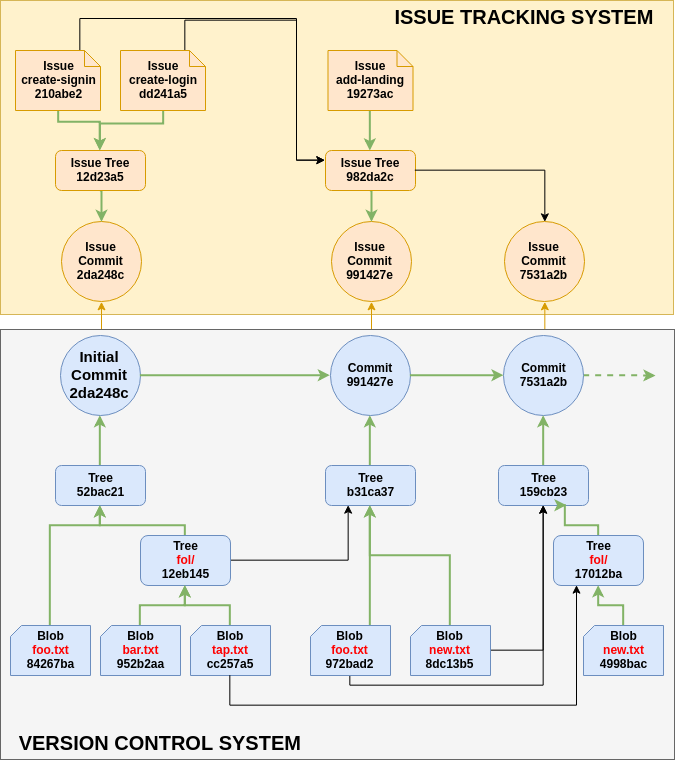
\includegraphics[width=10cm]{sciit-filesystem}
\end{figure}

% describe how issues are stored and managed

Each individual issue tree reference is attached to a special object called an issue commits. For all intents and purposes, they contain the reference to a git commit and a reference to an issue tree. This way they represent both the ITS and VCS creating one system that manages both activities. The resulting Source Control Integrated Issue Tracking (SCIIT) System can now be adequately used to represent the complex relationships between the management of issues and the state of the software project. Figure \ref{fig:sciit-filesystem} shows how SCIIT integrates the ITS alonside the VCS on the file system as a series references when commits are created.

As shown in Figure \ref{fig:sciit-filesystem} every commit made in git generates an issue commit that contains references to all the revisions made to those issues. This therefore poses a change in the traditional management of issues. If an issue is changed by editing the issue data embedded in the soruce code as a comment then a new issue object is created and assigned to a new issue tree. Changes to the references of an issue object over time can now be associated with a change in the issue. The issue tracker also intuitively determines if issues are closed by removing references to an issue that has been deleted from the embedded comment.

% how it works in a distributed environment

\section{Distributed Environments}

It is worth pointing out some design considerations of the system operation in a distributed environment since the backbone of the system is based on a distributed VCS. In Git, the main object of concern when it comes to a distributed environment is the branch. Each user has a local copy of the entire source code. They can make there changes locally and then push it to a remote repository where it can be merged with changes by other developer. In order to achieve such workflows branches are used. They represent a deviation from references to commits on other branches. Each has a HEAD which is the reference to the latest commit made on that branch. This way commits can now have different parents depending on which branch they belong to.

Although branching and merging, pushing and pulling are the main mechanisims allowing for distributed VCS, they all are based on the same primative object, the commit. Since our issue tracker was based on this primative object a branch from a commit will contain issue commits, issue trees and issues which may differ from other branches. This allows feature branches to contain feature specific issues. The utility of this design allows for the issue tracker to also be distributed in the sense that some issues can only be referenced from particular branches.

This concept gets compounded in merging senarios. In such events, developers can now be alerted by the VCS that there is a conflict with the issues as the full context of both referenced files are compared. At this point developer can decide in their pull request meetings or code reviews whether sufficient work has been done on the issue, if the issue is closed appropriately, or if to add more details in the issue for future development work. At merge points the primative commit object is saved and the SCIIT system will again scan for and update the issue tracker.

In a traditional sense however, issue trackers are meant to be a centralised system. Also if we consider that work is being done on a branch we should be able to capture all the information for all issues on all branches without conflicting data. Fortunately, git also allows for the querying of revisions such that all commits on all branches are returned maintaing thier parental links. The next chapter describes how this was implemented in order to maintain the valuable issue information on all branches.


% highlight the benefits achieved by the design

By maintaining issues in this manner we can see that a significant step has been taken to reduce the friction between the two development activities of maintaining the ITS and VCS. Developer now need only concern themselves with pulling, and pushing code to the repository where the issue tracker will seemlessly build, track and maintain issues in the background. This does not mean that developers are not resposible for looking at the embedded issues and performing the task it requires to implement them. However, it allows them to work in an environment with one point of contact. The design of SCIIT allows for developers to trod along writing code and to care for the issue tracking process. Additionally the issue tracker will now be up to date with the state of each revision of the source code.

The next sections will provide more details on how this was achieved and its practical use.

%%%%%%%%%%%%%%%%%%%%%%%%%%%%%%%%%%%%%%%%%%%%%%%%%%%%%%%%%%%%%%%%%%%%%%%%%%

\section{Implementation}

% talk about the git python library and how we intend to use this library to interface with the git objects in python
    % how the library was extended
    % 

% talk about how the git objects in python are manipulated to get the embedded issues

% talk about how the issues are saved to the file system and the references

% talk about the cli used to access the issues after they are created

% Hooks allow us to run custom scripts that perform issue management actions when particular git events take place.

\section{Challenges}

\section{Practical Use}
%%%%%%%%%%%%%%%%%%%%%%%%%%%%%%%%%%%%%%%%%%%%%%%%%%%%%%%%%%%%%%%%%%%
\chapter{Evaluation}\label{evaluation}

\section{Testing}


%%%%%%%%%%%%%%%%%%%%%%%%%%%%%%%%%%%%%%%%%%%%%%%%%%%%%%%%%%%%%%%%%%%
\chapter{Conclusion}\label{conclusion}

\section{Future Work}

\appendix % first appendix
%%%%%%%%%%%%%%%%%%%%%%%%%%%%%%%%%%%%%%%%%%%%%%%%%%%%%%%%%%%%%%%%%%%
\chapter{Development}

\section{Section of first appendix}

%%%%%%%%%%%%%%%%%%%%%%%%%%%%%%%%%%%%%%%%%%%%%%%%%%%%%%%%%%%%%%%%%%%
\chapter{Second appendix}

%%%%%%%%%%%%%%%%%%%%%%%%%%%%%%%%%%%%%%%%%%%%%%%%%%%%%%%%%%%%%%%%%%%
% it is fine to change the bibliography style if you want
\bibliographystyle{plain}
\bibliography{mproj}
\end{document}
